\documentclass[usenames,dvipsnames,tikz]{standalone}
%\usepackage{tikz}
%\usepackage{standalone}
\begin{document}
	
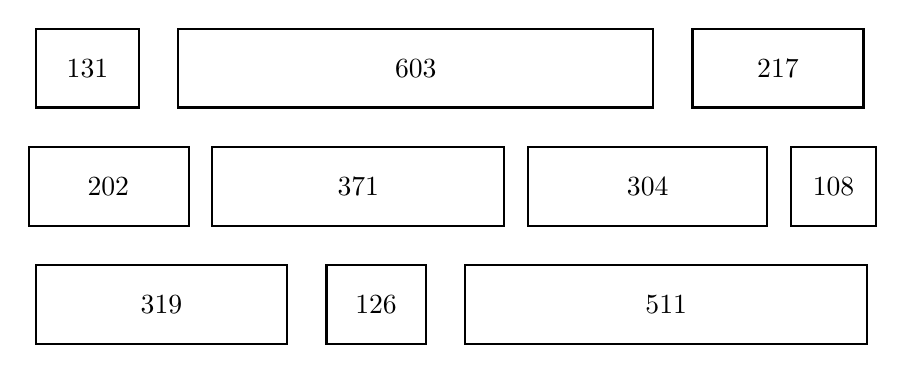
\begin{tikzpicture}
%\draw [help lines] (-1,-2) grid (13,11);


%------------------------------


%\draw [thick, white] (0,3.5) rectangle (10,4);
%\node at (5,-0.1) {\textcolor{white}{space}};

\draw [thick] (0,3) rectangle (1.31, 4); %131
\draw [thick] (1.81,3) rectangle (7.84, 4); %603
\draw [thick] (8.34,3) rectangle (10.51, 4); %217

\node at (0.655,3.5) {131};
\node at (4.825,3.5) {603};
\node at (9.425,3.5) {217};


\draw [thick] (-0.09,1.5) rectangle (1.94, 2.5); %202
\draw [thick] (2.24,1.5) rectangle (5.95, 2.5); %371
\draw [thick] (6.25,1.5) rectangle (9.29, 2.5); %304
\draw [thick] (9.59,1.5) rectangle (10.67, 2.5); %108
\node at (0.92,2) {202};
\node at (4.095,2) {371};
\node at (7.77,2) {304};
\node at (10.13,2) {108};


\draw [thick] (0,0) rectangle (3.19, 1); %319
\draw [thick] (3.69,0) rectangle (4.95, 1); %126
\draw [thick] (5.45,0) rectangle (10.56, 1); %511
\node at (1.595,0.5) {319};
\node at (4.32,0.5) {126};
\node at (8.005,0.5) {511};

%---------------------
%Smaller height of items.

%BLANK BINS TO MATCH BPP.TEX
%\draw [thick, white] (0,0) rectangle (10,0.75); %bottom row
%\draw [thick, white] (0,1.25) rectangle (10,2); %middle row
%\draw [thick, white] (0,2.5) rectangle (10,3.25); %top row

%------------------------

%\draw [thick, white] (0,3.5) rectangle (10,4);
%\node at (5,-0.1) {\textcolor{white}{space}};

%\draw [thick] (0,2.5) rectangle (1.31, 3.25); %131
%\draw [thick] (1.81,2.5) rectangle (7.84, 3.25); %603
%\draw [thick] (8.34,2.5) rectangle (10.85, 3.25); %251
%%\draw [thick, dashed] (0.17,3) -- (0.17,4);
%%\draw [thick, dashed] (2.83,3) -- (2.83,4);
%%\draw [thick, dashed] (3.99,3) -- (3.99,4);
%%\draw [thick, dashed] (5.01,3) -- (5.01,4);
%%\draw [thick, dashed] (6.67,3) -- (6.67,4);
%%\draw [thick, dashed] (11.17,3) -- (11.17,4);
%\node at (0.655,2.875) {131};
%\node at (4.825,2.875) {603};
%\node at (9.595,2.875) {251};
%
%
%\draw [thick] (-0.07,1.25) rectangle (1.96, 2); %202
%\draw [thick] (2.26,1.25) rectangle (6.23, 2); %397
%\draw [thick] (6.53,1.25) rectangle (9.67, 2); %314
%\draw [thick] (9.97,1.25) rectangle (11.03, 2); %106
%%\draw [thick, dashed] (0.1,1.5) -- (0.1,2.5);
%%\draw [thick, dashed] (4.83,1.5) -- (4.83,2.5);
%%\draw [thick, dashed] (5.88,1.5) -- (5.88,2.5);
%%\draw [thick, dashed] (8.49,1.5) -- (8.49,2.5);
%%\draw [thick, dashed] (9.94,1.5) -- (9.94,2.5);
%%\draw [thick, dashed] (10.84,1.5) -- (10.84,2.5);
%\node at (0.95,1.625) {202};
%\node at (4.245,1.625) {397};
%\node at (8.1,1.625) {314};
%\node at (10.5,1.625) {106};
%
%
%\draw [thick] (0,0) rectangle (3.47, 0.75); %347
%\draw [thick] (3.97,0) rectangle (5.24, 0.75); %127
%\draw [thick] (5.74,0) rectangle (10.96, 0.75); %522
%%\draw [thick, dashed] (0.16,0) -- (0.16,1);
%%\draw [thick, dashed] (2.97,0) -- (2.97,1);
%%\draw [thick, dashed] (4.04,0) -- (4.04,1);
%%\draw [thick, dashed] (7,0) -- (7,1);
%%\draw [thick, dashed] (8.3,0) -- (8.3,1);
%%\draw [thick, dashed] (10.76,0) -- (10.76,1);
%\node at (1.735,0.375) {347};
%\node at (4.605,0.375) {127};
%\node at (8.35,0.375) {522};





\end{tikzpicture}
	
\end{document}